% Options for packages loaded elsewhere
\PassOptionsToPackage{unicode}{hyperref}
\PassOptionsToPackage{hyphens}{url}
%
\documentclass[
  8pt,
  ignorenonframetext,
]{beamer}
\usepackage{pgfpages}
\setbeamertemplate{caption}[numbered]
\setbeamertemplate{caption label separator}{: }
\setbeamercolor{caption name}{fg=normal text.fg}
\beamertemplatenavigationsymbolsempty
% Prevent slide breaks in the middle of a paragraph
\widowpenalties 1 10000
\raggedbottom
\setbeamertemplate{part page}{
  \centering
  \begin{beamercolorbox}[sep=16pt,center]{part title}
    \usebeamerfont{part title}\insertpart\par
  \end{beamercolorbox}
}
\setbeamertemplate{section page}{
  \centering
  \begin{beamercolorbox}[sep=12pt,center]{part title}
    \usebeamerfont{section title}\insertsection\par
  \end{beamercolorbox}
}
\setbeamertemplate{subsection page}{
  \centering
  \begin{beamercolorbox}[sep=8pt,center]{part title}
    \usebeamerfont{subsection title}\insertsubsection\par
  \end{beamercolorbox}
}
\AtBeginPart{
  \frame{\partpage}
}
\AtBeginSection{
  \ifbibliography
  \else
    \frame{\sectionpage}
  \fi
}
\AtBeginSubsection{
  \frame{\subsectionpage}
}
\usepackage{amsmath,amssymb}
\usepackage{lmodern}
\usepackage{iftex}
\ifPDFTeX
  \usepackage[T1]{fontenc}
  \usepackage[utf8]{inputenc}
  \usepackage{textcomp} % provide euro and other symbols
\else % if luatex or xetex
  \usepackage{unicode-math}
  \defaultfontfeatures{Scale=MatchLowercase}
  \defaultfontfeatures[\rmfamily]{Ligatures=TeX,Scale=1}
\fi
% Use upquote if available, for straight quotes in verbatim environments
\IfFileExists{upquote.sty}{\usepackage{upquote}}{}
\IfFileExists{microtype.sty}{% use microtype if available
  \usepackage[]{microtype}
  \UseMicrotypeSet[protrusion]{basicmath} % disable protrusion for tt fonts
}{}
\makeatletter
\@ifundefined{KOMAClassName}{% if non-KOMA class
  \IfFileExists{parskip.sty}{%
    \usepackage{parskip}
  }{% else
    \setlength{\parindent}{0pt}
    \setlength{\parskip}{6pt plus 2pt minus 1pt}}
}{% if KOMA class
  \KOMAoptions{parskip=half}}
\makeatother
\usepackage{xcolor}
\newif\ifbibliography
\usepackage{color}
\usepackage{fancyvrb}
\newcommand{\VerbBar}{|}
\newcommand{\VERB}{\Verb[commandchars=\\\{\}]}
\DefineVerbatimEnvironment{Highlighting}{Verbatim}{commandchars=\\\{\}}
% Add ',fontsize=\small' for more characters per line
\usepackage{framed}
\definecolor{shadecolor}{RGB}{248,248,248}
\newenvironment{Shaded}{\begin{snugshade}}{\end{snugshade}}
\newcommand{\AlertTok}[1]{\textcolor[rgb]{0.94,0.16,0.16}{#1}}
\newcommand{\AnnotationTok}[1]{\textcolor[rgb]{0.56,0.35,0.01}{\textbf{\textit{#1}}}}
\newcommand{\AttributeTok}[1]{\textcolor[rgb]{0.77,0.63,0.00}{#1}}
\newcommand{\BaseNTok}[1]{\textcolor[rgb]{0.00,0.00,0.81}{#1}}
\newcommand{\BuiltInTok}[1]{#1}
\newcommand{\CharTok}[1]{\textcolor[rgb]{0.31,0.60,0.02}{#1}}
\newcommand{\CommentTok}[1]{\textcolor[rgb]{0.56,0.35,0.01}{\textit{#1}}}
\newcommand{\CommentVarTok}[1]{\textcolor[rgb]{0.56,0.35,0.01}{\textbf{\textit{#1}}}}
\newcommand{\ConstantTok}[1]{\textcolor[rgb]{0.00,0.00,0.00}{#1}}
\newcommand{\ControlFlowTok}[1]{\textcolor[rgb]{0.13,0.29,0.53}{\textbf{#1}}}
\newcommand{\DataTypeTok}[1]{\textcolor[rgb]{0.13,0.29,0.53}{#1}}
\newcommand{\DecValTok}[1]{\textcolor[rgb]{0.00,0.00,0.81}{#1}}
\newcommand{\DocumentationTok}[1]{\textcolor[rgb]{0.56,0.35,0.01}{\textbf{\textit{#1}}}}
\newcommand{\ErrorTok}[1]{\textcolor[rgb]{0.64,0.00,0.00}{\textbf{#1}}}
\newcommand{\ExtensionTok}[1]{#1}
\newcommand{\FloatTok}[1]{\textcolor[rgb]{0.00,0.00,0.81}{#1}}
\newcommand{\FunctionTok}[1]{\textcolor[rgb]{0.00,0.00,0.00}{#1}}
\newcommand{\ImportTok}[1]{#1}
\newcommand{\InformationTok}[1]{\textcolor[rgb]{0.56,0.35,0.01}{\textbf{\textit{#1}}}}
\newcommand{\KeywordTok}[1]{\textcolor[rgb]{0.13,0.29,0.53}{\textbf{#1}}}
\newcommand{\NormalTok}[1]{#1}
\newcommand{\OperatorTok}[1]{\textcolor[rgb]{0.81,0.36,0.00}{\textbf{#1}}}
\newcommand{\OtherTok}[1]{\textcolor[rgb]{0.56,0.35,0.01}{#1}}
\newcommand{\PreprocessorTok}[1]{\textcolor[rgb]{0.56,0.35,0.01}{\textit{#1}}}
\newcommand{\RegionMarkerTok}[1]{#1}
\newcommand{\SpecialCharTok}[1]{\textcolor[rgb]{0.00,0.00,0.00}{#1}}
\newcommand{\SpecialStringTok}[1]{\textcolor[rgb]{0.31,0.60,0.02}{#1}}
\newcommand{\StringTok}[1]{\textcolor[rgb]{0.31,0.60,0.02}{#1}}
\newcommand{\VariableTok}[1]{\textcolor[rgb]{0.00,0.00,0.00}{#1}}
\newcommand{\VerbatimStringTok}[1]{\textcolor[rgb]{0.31,0.60,0.02}{#1}}
\newcommand{\WarningTok}[1]{\textcolor[rgb]{0.56,0.35,0.01}{\textbf{\textit{#1}}}}
\setlength{\emergencystretch}{3em} % prevent overfull lines
\providecommand{\tightlist}{%
  \setlength{\itemsep}{0pt}\setlength{\parskip}{0pt}}
\setcounter{secnumdepth}{-\maxdimen} % remove section numbering
\newlength{\cslhangindent}
\setlength{\cslhangindent}{1.5em}
\newlength{\csllabelwidth}
\setlength{\csllabelwidth}{3em}
\newlength{\cslentryspacingunit} % times entry-spacing
\setlength{\cslentryspacingunit}{\parskip}
\newenvironment{CSLReferences}[2] % #1 hanging-ident, #2 entry spacing
 {% don't indent paragraphs
  \setlength{\parindent}{0pt}
  % turn on hanging indent if param 1 is 1
  \ifodd #1
  \let\oldpar\par
  \def\par{\hangindent=\cslhangindent\oldpar}
  \fi
  % set entry spacing
  \setlength{\parskip}{#2\cslentryspacingunit}
 }%
 {}
\usepackage{calc}
\newcommand{\CSLBlock}[1]{#1\hfill\break}
\newcommand{\CSLLeftMargin}[1]{\parbox[t]{\csllabelwidth}{#1}}
\newcommand{\CSLRightInline}[1]{\parbox[t]{\linewidth - \csllabelwidth}{#1}\break}
\newcommand{\CSLIndent}[1]{\hspace{\cslhangindent}#1}
% type setting
% ------------------------------------------------------------------------------
\usepackage[german]{babel}     

% fonts
% ------------------------------------------------------------------------------
\usefonttheme{professionalfonts}

% slide title and horizontal line
% ------------------------------------------------------------------------------
\setbeamertemplate{frametitle}{%
    \vskip-30pt \color{black}\large%
    \begin{minipage}[b][23pt]{120mm}%
    \flushleft\insertframetitle%
    \end{minipage}%
}

\setbeamertemplate{headline}										
{
\vskip10pt\hfill\hspace{3.5mm} 										 
\vskip15pt\color{black}\rule{\textwidth}{0.4pt} 					 
}

% slide number
% ---------------------------------------------------------------
\setbeamertemplate{navigation symbols}{}
\setbeamertemplate{footline}
{
\vskip5pt
\vskip2pt
\makebox[123mm]{\hspace{7.5mm}
\hfill Allgemeines Lineares Modell $\vert$ 
\copyright $ $ 2023 Dirk Ostwald CC BY 4.0 $\vert$ 
Folie \insertframenumber}
\vskip4pt
}

% block color scheme
% ------------------------------------------------------------------------------
% colors
\definecolor{white}{RGB}{255,255,255}
\definecolor{grey}{RGB}{235,235,235}
\definecolor{lightgrey}{RGB}{245,245,245}
\definecolor{LightBlue}{RGB}{220,220,255}
\definecolor{darkblue}{RGB}{51, 51, 153}

% definitions and theorems
\setbeamercolor{block title}{fg = black, bg = grey}
\setbeamercolor{block body}{fg = black, bg = lightgrey}

% general line spacing 
% ------------------------------------------------------------------------------
\linespread{1.3}

% local line spacing
% ------------------------------------------------------------------------------
\usepackage{setspace}

% colors
% -----------------------------------------------------------------------------
\usepackage{color}

% justified text
% ------------------------------------------------------------------------------
\usepackage{ragged2e}
\usepackage{etoolbox}
\apptocmd{\frame}{}{\justifying}{}

% bullet point lists
% -----------------------------------------------------------------------------
\setbeamertemplate{itemize item}[circle]
\setbeamertemplate{itemize subitem}[circle]
\setbeamertemplate{itemize subsubitem}[circle]
\setbeamercolor{itemize item}{fg = black}
\setbeamercolor{itemize subitem}{fg = black}
\setbeamercolor{itemize subsubitem}{fg = black}
\setbeamercolor{enumerate item}{fg = black}
\setbeamercolor{enumerate subitem}{fg = black}
\setbeamercolor{enumerate subsubitem}{fg = black}
\setbeamerfont{itemize/enumerate body}{}
\setbeamerfont{itemize/enumerate subbody}{size = \normalsize}
\setbeamerfont{itemize/enumerate subsubbody}{size = \normalsize}

% color links
% ------------------------------------------------------------------------------
\usepackage{hyperref}
\definecolor{urls}{RGB}{204,0,0}
\hypersetup{colorlinks, citecolor = darkblue, urlcolor = urls}


% additional math commands
% ------------------------------------------------------------------------------
\usepackage{bm}     
\newcommand{\niton}{\not\owns}
\DeclareMathOperator*{\intinf}{\int_{-\infty}^{\infty}}
\DeclareSymbolFont{extraitalic}      {U}{zavm}{m}{it}
\DeclareMathSymbol{\Qoppa}{\mathord}{extraitalic}{161}
\DeclareMathSymbol{\qoppa}{\mathord}{extraitalic}{162}

% text highlighting
% ------------------------------------------------------------------------------
\usepackage{soul}
\makeatletter
\let\HL\hl
\renewcommand\hl{%
  \let\set@color\beamerorig@set@color
  \let\reset@color\beamerorig@reset@color
  \HL}
\makeatother

% equation highlighting
% -----------------------------------------------------------------------------
\newcommand{\highlight}[2][yellow]{\mathchoice%
  {\colorbox{#1}{$\displaystyle#2$}}%
  {\colorbox{#1}{$\textstyle#2$}}%
  {\colorbox{#1}{$\scriptstyle#2$}}%
  {\colorbox{#1}{$\scriptscriptstyle#2$}}}%

% additional mathematical operators
% ------------------------------------------------------------------------------
\DeclareMathOperator*{\argmax}{arg\,max}
\DeclareMathOperator*{\argmin}{arg\,min}

\ifLuaTeX
  \usepackage{selnolig}  % disable illegal ligatures
\fi
\IfFileExists{bookmark.sty}{\usepackage{bookmark}}{\usepackage{hyperref}}
\IfFileExists{xurl.sty}{\usepackage{xurl}}{} % add URL line breaks if available
\urlstyle{same} % disable monospaced font for URLs
\hypersetup{
  hidelinks,
  pdfcreator={LaTeX via pandoc}}

\author{}
\date{\vspace{-2.5em}}

\begin{document}

\begin{frame}[plain]{}
\protect\hypertarget{section}{}
\center

\begin{center}
\includegraphics[width=0.2\linewidth]{8_Abbildungen/alm_8_otto} \end{center}

\vspace{2mm}

\huge

Allgemeines Lineares Modell \vspace{6mm}

\large

BSc Psychologie SoSe 2023

\vspace{6mm}
\normalsize

Prof.~Dr.~Dirk Ostwald
\end{frame}

\begin{frame}[plain]{}
\protect\hypertarget{section-1}{}
\center
\huge
\vfill

\noindent (8) F-Statistiken \vfill
\end{frame}

\begin{frame}{}
\protect\hypertarget{section-2}{}
\large

Naturwissenschaft \vspace{7mm}

\begin{center}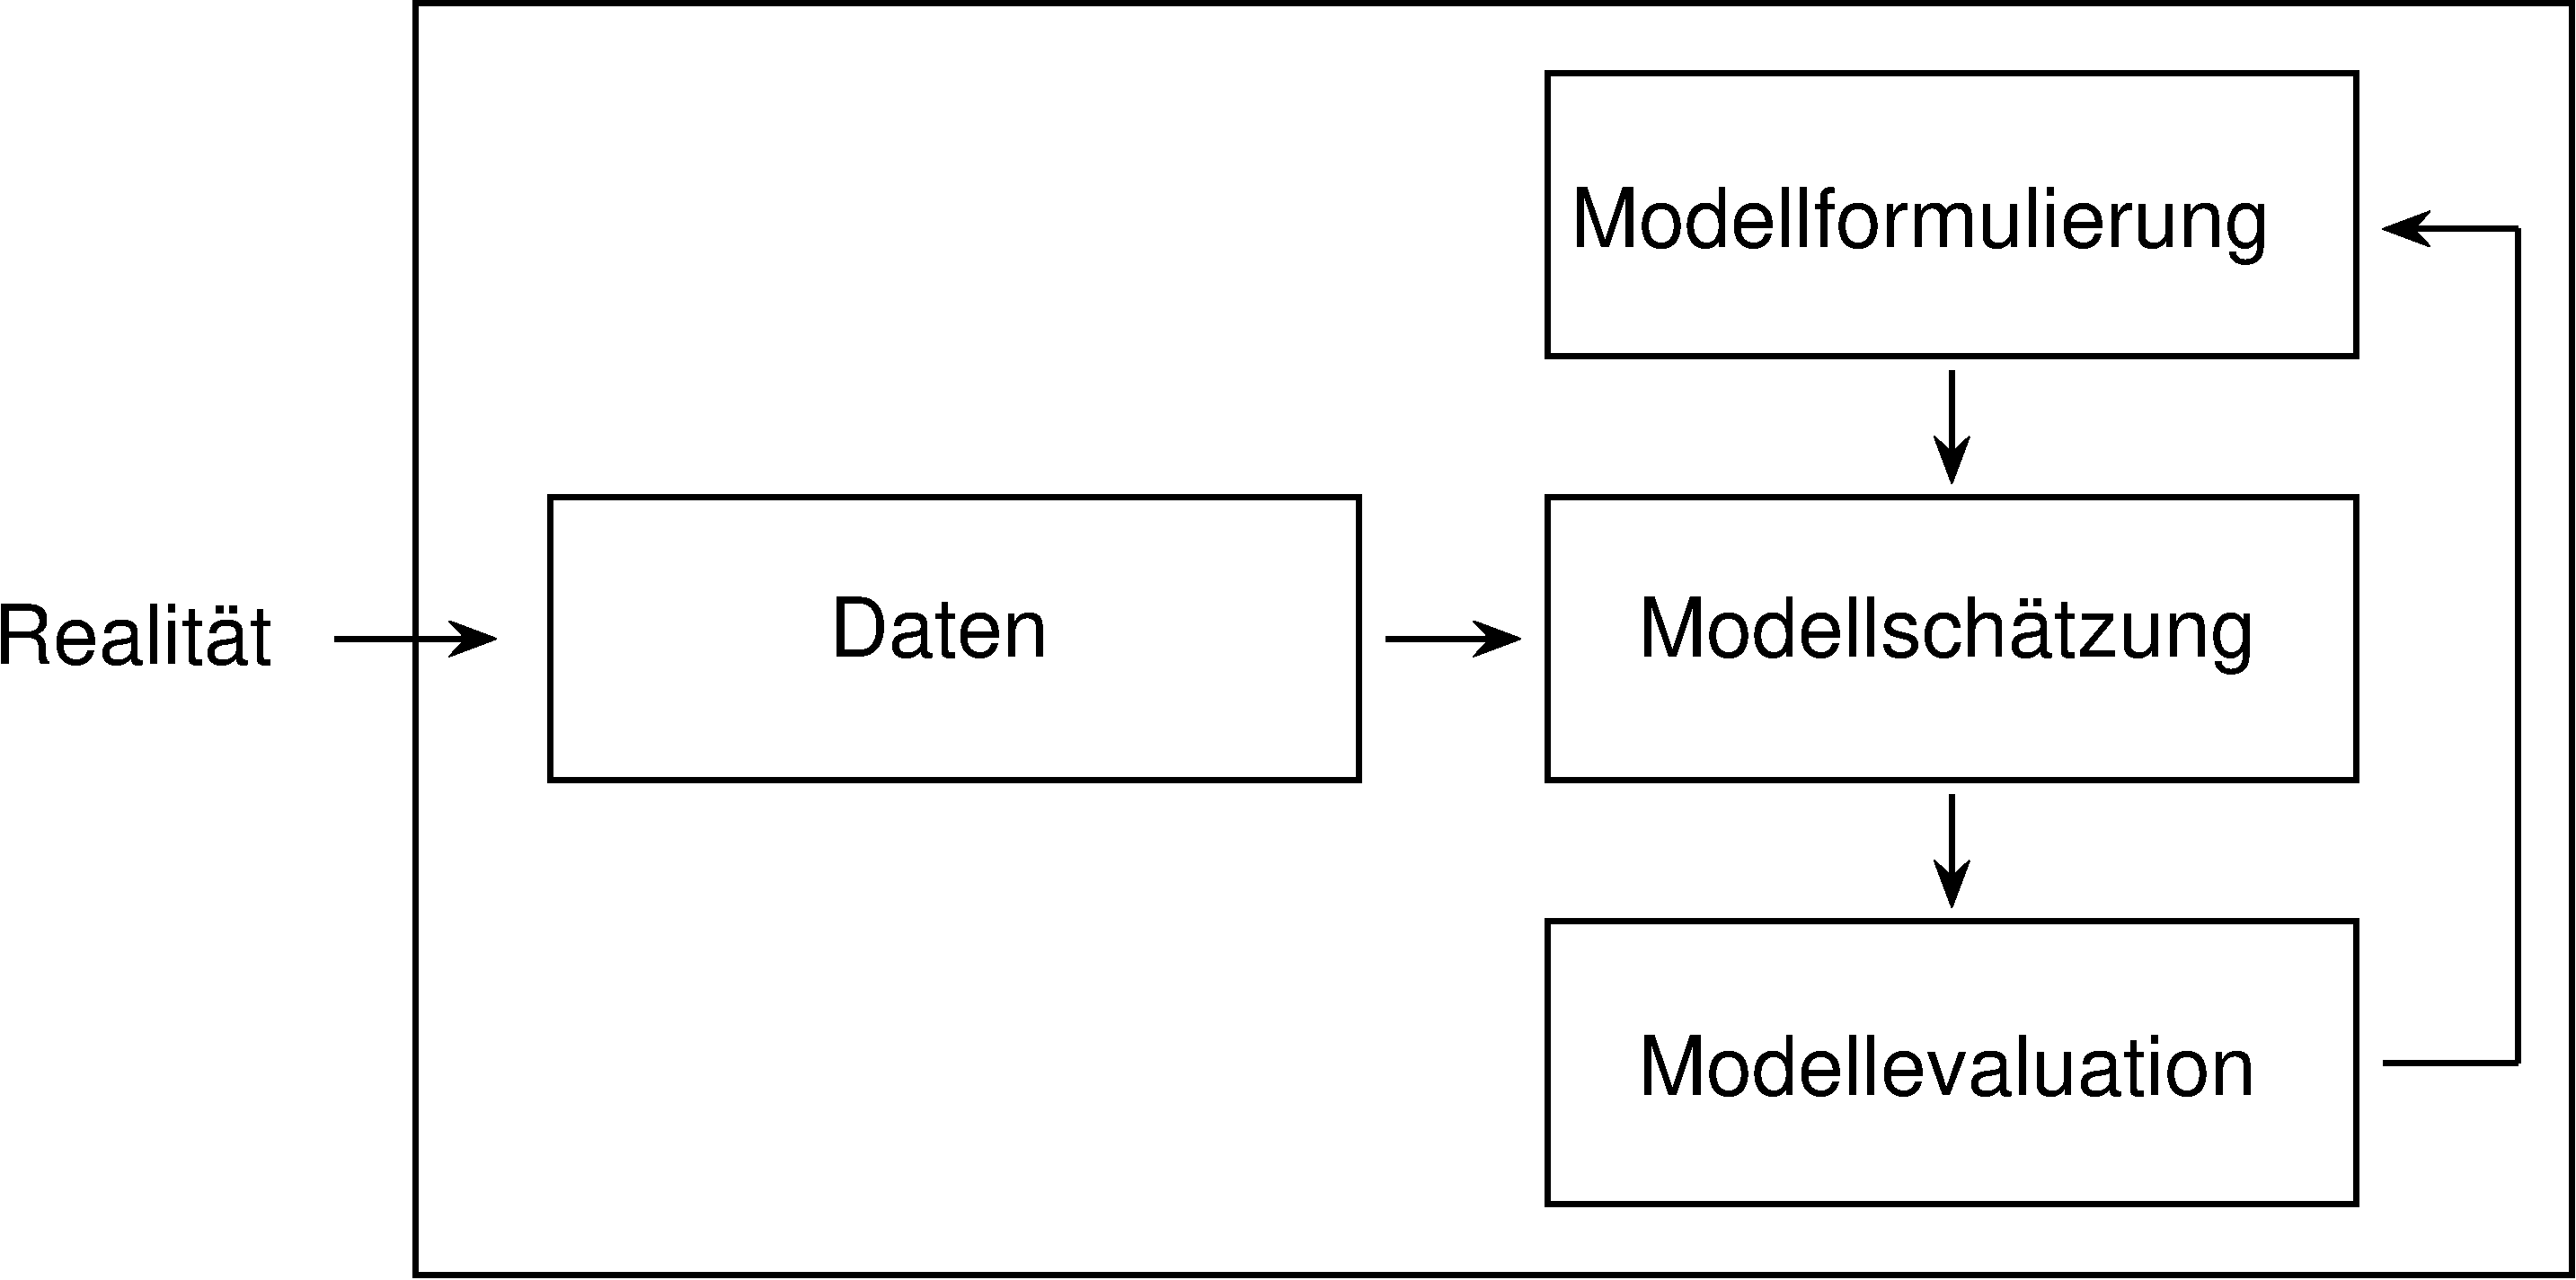
\includegraphics[width=0.9\linewidth]{8_Abbildungen/alm_8_wissenschaft} \end{center}
\end{frame}

\begin{frame}{}
\protect\hypertarget{section-3}{}
\vspace{1mm}
\normalsize

Modellformulierung \vspace{1mm} \small \begin{equation}
\upsilon = X\beta + \varepsilon, \varepsilon \sim N(0_n,\sigma^2I_n)
\end{equation} \vspace{5mm}

\normalsize

Modellschätzung \small \begin{equation}
\hat{\beta} = (X^TX)^{-1} X^T\upsilon,  \hat{\sigma}^2 = \frac{(\upsilon-X\hat{\beta})^T(\upsilon-X\hat{\beta})}{n-p}
\end{equation} \vspace{4mm}

\normalsize

Modellevaluation \small \begin{equation}
T = \frac{c^T\hat{\beta} - c^T\beta_0}{\sqrt{\hat{\sigma}^2c^T(X^TX)^{-1}c}},
F = \frac{(\hat{\varepsilon}_0^T\hat{\varepsilon}_0 - \hat{\varepsilon}^T\hat{\varepsilon})/p_1}{\hat{\varepsilon}^T\hat{\varepsilon}/(n-p)}
\end{equation}
\end{frame}

\begin{frame}{}
\protect\hypertarget{section-4}{}
Standardprobleme Frequentistischer Inferenz

\small
\vspace{2mm}

\noindent (1) Parameterschätzung

Ziel der Parameterschätzung ist es, einen möglichst guten Tipp für
wahre, aber unbekannte, Parameterwerte oder Funktionen dieser abzugeben,
typischerweise mithilfe von Daten.

\vspace{2mm}

\noindent (2) Konfidenzintervalle

Ziel der Bestimmung von Konfidenzintervallen ist es, basierend auf der
angenommenen Verteilung der Daten eine quantitative Aussage über die mit
Schätzwerten assoziierte Unsicherheit zu treffen.

\vspace{2mm}

\noindent (3) Hypothesentests

Ziel des Hypothesentestens ist es, basierend auf der angenommenen
Verteilung der Daten in einer möglichst zuverlässigen Form zu
entscheiden, ob ein wahrer, aber unbekannter Parameterwert in einer von
zwei sich gegenseitig ausschließenden Untermengen des Parameterraumes
liegt.
\end{frame}

\begin{frame}{}
\protect\hypertarget{section-5}{}
\center

\begin{center}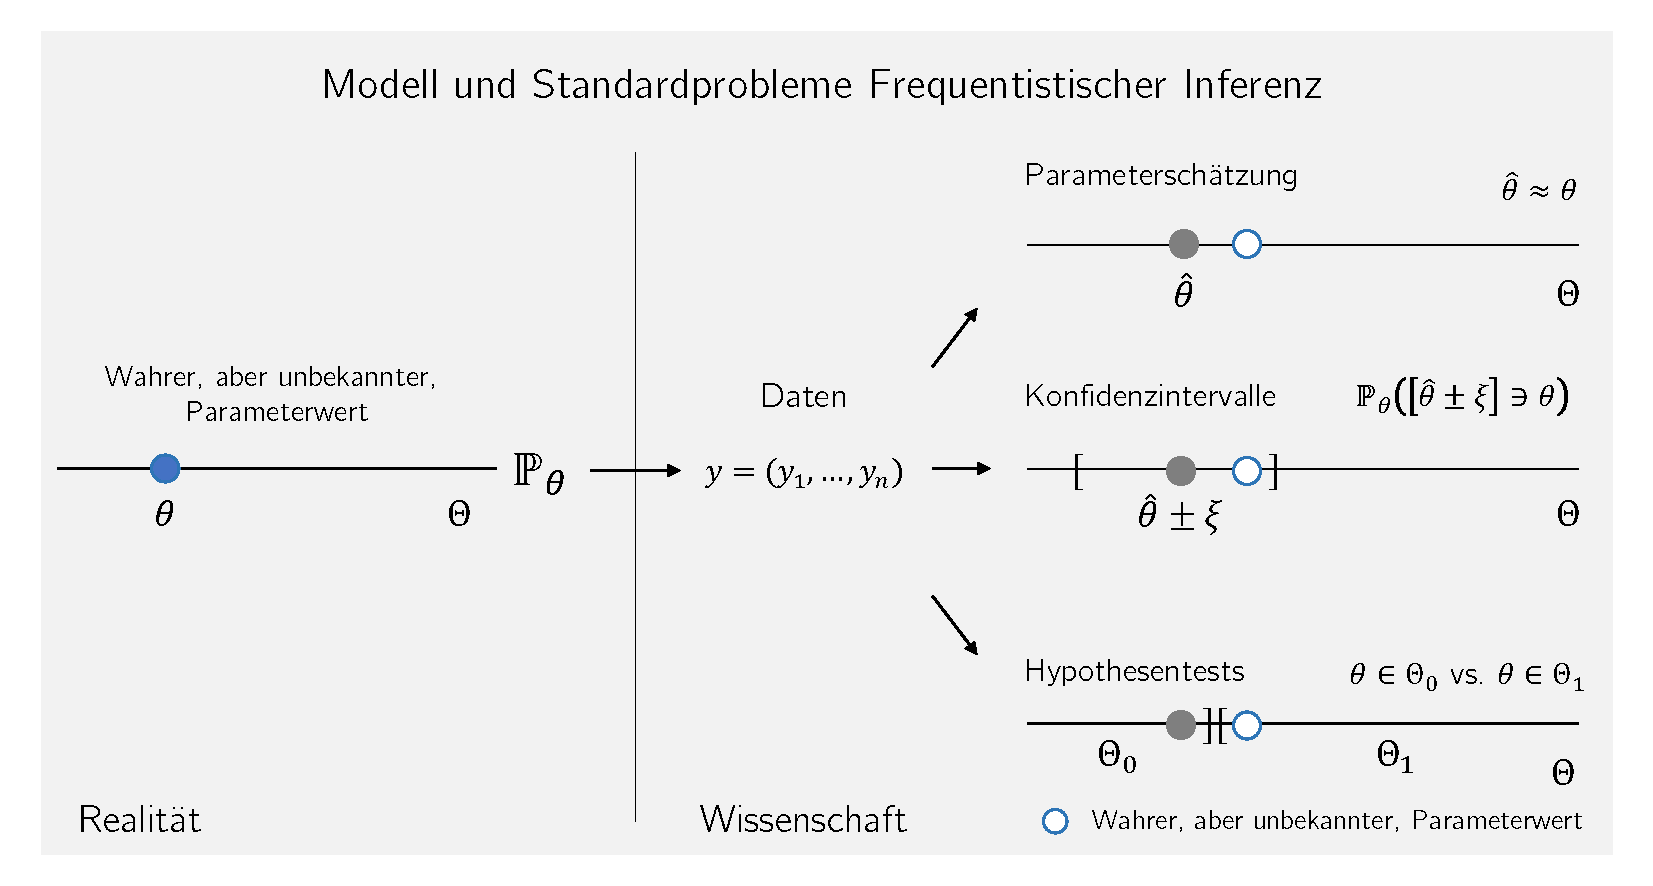
\includegraphics[width=1\linewidth]{8_Abbildungen/alm_8_frequentistische_inferenz} \end{center}
\center
\footnotesize

\(\theta := (\beta,\sigma^2)\),
\(\Theta := \mathbb{R}^p \times \mathbb{R}_{>0}\)
\(\mathbb{P}_\theta(\upsilon) := \mathbb{P}_{\beta,\sigma^2}(\upsilon)\)
mit WDF \(p_{\beta,\sigma^2}(y) := N(y;X\beta,\sigma^2I_n)\)
\end{frame}

\begin{frame}{}
\protect\hypertarget{section-6}{}
\small

Standardannahmen Frequentistischer Inferenz

\footnotesize
\setstretch{1.2}

Gegeben sei das Allgemeine Lineare Modell. Es wird angenommen, dass ein
vorliegender Datensatz eine der möglichen Realisierungen der Daten des
Modells ist. Aus Frequentistischer Sicht kann man unendlich oft
Datensätze basierend auf einem Modell generieren und zu jedem Datensatz
Schätzer oder Statistiken auswerten, z.B. den Betaparameterschätzer
\vspace{1mm}

\begin{itemize}
\item[] Datensatz (1) : $y^{(1)} = \left(y_1^{(1)}, y_2^{(1)}, ...,y_n^{(1)}\right)^T$  mit $\hat{\beta}^{(1)} = (X^TX)^{-1}X^Ty^{(1)}$
\item[] Datensatz (2) : $y^{(2)} = \left(y_1^{(2)}, y_2^{(2)}, ...,y_n^{(2)}\right)^T$  mit $\hat{\beta}^{(2)} = (X^TX)^{-1}X^Ty^{(2)}$
\item[] Datensatz (3) : $y^{(3)} = \left(y_1^{(3)}, y_2^{(3)}, ...,y_n^{(3)}\right)^T$  mit $\hat{\beta}^{(3)} = (X^TX)^{-1}X^Ty^{(3)}$
\item[] Datensatz (4) : $y^{(4)} = \left(y_1^{(4)}, y_2^{(4)}, ...,y_n^{(4)}\right)^T$  mit $\hat{\beta}^{(4)} = (X^TX)^{-1}X^Ty^{(4)}$
\item[] Datensatz (5) : $y^{(5)} = ...$
\end{itemize}

\vspace{1mm}

Um die Qualität statistischer Methoden zu beurteilen betrachtet die
Frequentistische Statistik die Wahrscheinlichkeitsverteilungen von
Schätzern und Statistiken unter Annahme der Datenverteilung. Was zum
Beispiel ist die Verteilung von \(\hat{\beta}^{(1)}\),
\(\hat{\beta}^{(2)}\), \(\hat{\beta}^{(3)}\), \(\hat{\beta}^{(4)}\),
\ldots{} also die Verteilung der Zufallsvariable
\(\hat{\beta} := (X^TX)^{-1}X^T\upsilon\)? Wenn eine statistische
Methode im Sinne der Frequentistischen Standardannahmen ``gut'' ist,
dann heißt das also, dass sie bei häufiger Anwendung ``im Mittel gut''
ist. Im Einzelfall, also im Normalfall nur eines vorliegenden
Datensatzes, kann sie auch ``schlecht'' sein.
\end{frame}

\begin{frame}{}
\protect\hypertarget{section-7}{}
\small

Überblick

\begin{itemize}
\item
  \justifying Wir führen F-Statistiken hier vor dem Hintergrund
  Likelihood-Quotienten-basierter Modellvergleiche ein. Die (maximierte
  oder marginale) Likelihood eines Datensatzes unter einem gegebenen
  probabilistischen Modell als Modellvergleichskriterium heranzuziehen
  ist ein weit verbreitetes Verfahren in der probabilistischen
  Datenanalyse.
\item
  \justifying Im Gegensatz zu T-Statistiken kann das Ziel der Berechnung
  von F-Statistiken damit insbesondere sein, nicht nur
  Linearkombinationen von Betaparameterschätzwerten probabilistisch zu
  evaluieren, sondern die Modellanpassung an einen Datensatz insgesamt
  zu evaluieren.
\item
  \justifying Die Modellvergleichskapazität von F-Statistiken ist
  allerdings etwas beschränkt, da sich die F-Statistik nur auf ALMs und
  insbesondere geschachtelte ALMs bezieht, in denen ein Modell
  Bestandteil eines anderen Modells ist.
\item
  \justifying F-Statistiken bilden üblicherweise die Grundlage für
  Hypothesentests im Rahmen varianzanalytischer Verfahren (vgl. (10)
  Einfaktorielle Varianzanalyse, (11) Zweifaktorielle Varianzanalyse und
  (13) Kovarianzanalyse). Der Einsatz von F-Statistiken ist aber
  \emph{perse} nicht auf Varianzanalysen beschränkt, sondern kann auch
  bei parametrischen ALM Designs angebracht sein.
\end{itemize}
\end{frame}

\begin{frame}{}
\protect\hypertarget{section-8}{}
\vfill
\large
\setstretch{3}

F-Zufallsvariablen

Likelihood-Quotienten

Definition und Verteilung

Selbstkontrollfragen \vfill
\end{frame}

\begin{frame}{}
\protect\hypertarget{section-9}{}
\vfill
\large
\setstretch{3}

\textbf{F-Zufallsvariablen}

Likelihood-Quotienten

Definition und Verteilung

Selbstkontrollfragen \vfill
\end{frame}

\begin{frame}{F-Zufallsvariablen}
\protect\hypertarget{f-zufallsvariablen}{}
\footnotesize
\begin{definition}[$f$-Zufallsvariable]
\justifying
$\xi$ sei eine Zufallsvariable mit Ergebnisraum $\mathbb{R}_{>0}$ und Wahrscheinlichkeitsdichtefunktion
\begin{equation}
p_\xi : \mathbb{R} \to \mathbb{R}_{>0}, x \mapsto p_\xi(x)
:= \nu_1^{\frac{\nu_1}{2}}\nu_2^{\frac{\nu_2}{2}}
   \frac{\Gamma\left(\frac{\nu_1+\nu_2}{2}\right)}{\Gamma\left(\frac{\nu_1}{2}\right)\Gamma\left(\frac{\nu_2}{2}\right)}
   \frac{x^{\frac{\nu_1}{2}-1}}{\left(\nu_1 x  + \nu_2 \right)^{\frac{\nu_1+\nu_2}{2}}},
\end{equation}
wobei $\Gamma$ die Gammafunktion bezeichne. Dann sagen wir, dass $\xi$ einer
$f$-Verteilung mit Freiheitsgradparametern $\nu_1$ und $\nu_2$ unterliegt und nennen $\xi$ eine
$f$-Zufallsvariable mit Freiheitsgradparametern $\nu_1$ und $\nu_2$. Wir kürzen dies
mit $\xi \sim f(\nu_1,\nu_2)$ ab. Die Wahrscheinlichkeitsdichtefunktion (WDF) einer
$f$-Zufallsvariable bezeichnen wir mit $f(x;\nu_1,\nu_2)$, die kumulative Verteilungsfunktion (KVF)
einer $f$-Zufallsvariable bezeichnen wir mit $\varphi(x;\nu_1,\nu_2)$, und die inverse
kumulative Verteilungsfunktion einer $f$-Zufallsvariable bezeichnen wir mit $\varphi^{-1}(x;\nu_1,\nu_2)$.
\end{definition}

Bemerkungen

\begin{itemize}
\tightlist
\item
  \(f\)-Zufallsvariablen sind nach Ronald A. Fisher benannt.
\item
  George W. Snedecor hat die KVF der \(f\)-Verteilung wohl 1934
  basierend auf Arbeiten von Fisher tabuliert.
\end{itemize}
\end{frame}

\begin{frame}{F-Zufallsvariablen}
\protect\hypertarget{f-zufallsvariablen-1}{}
\vfill

\small

Wahrscheinlichkeitsdichtefunktionen von \(f\)-Verteilungen \vspace{1mm}

\begin{center}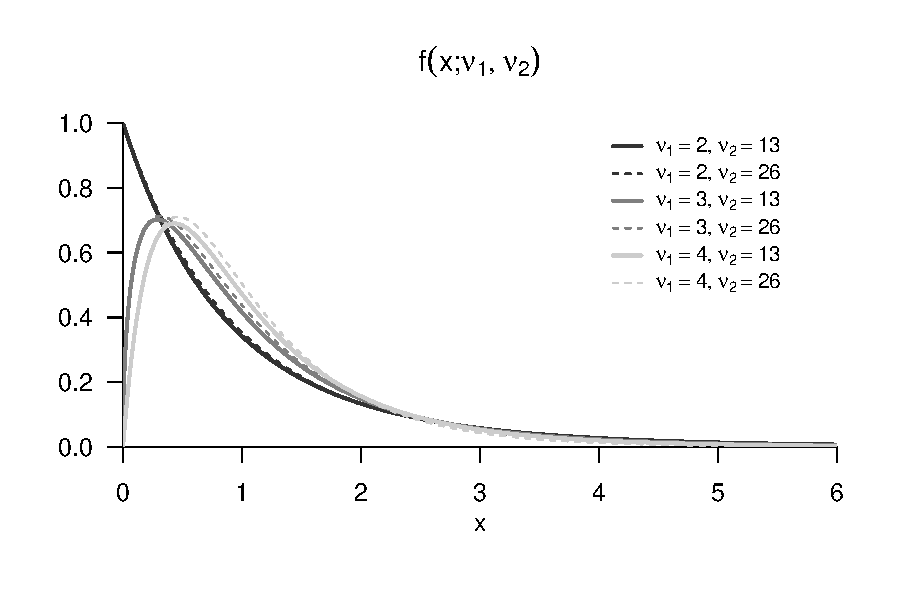
\includegraphics[width=0.8\linewidth]{8_Abbildungen/alm_8_f_wdf} \end{center}
\end{frame}

\begin{frame}{F-Zufallsvariablen}
\protect\hypertarget{f-zufallsvariablen-2}{}
\small
\begin{theorem}[$F$-Transformation]
\justifying
\normalfont
$\zeta_1 \sim \chi^2(\nu_1)$ und $\zeta_2 \sim \chi^2(\nu_2)$ seien zwei unabhängige
$\chi^2$-Zufallfsvariablen mit $\nu_1$ und $\nu_2$ Freiheitsgraden, respektive.
Dann ist die Zufallsvariable
\begin{equation}
\xi := \frac{\zeta_1/\nu_1}{\zeta_2/\nu_2}
\end{equation}
eine $f$-verteilte Zufallsvariable mit $\nu_1,\nu_2$ Freiheitsgraden, es gilt also $\xi \sim f(\nu_1,\nu_2)$.
\end{theorem}

\footnotesize

Bemerkungen

\begin{itemize}
\tightlist
\item
  Wir verzichten auf einen Beweis.
\item
  Das Theorem kann bewiesen werden, in dem man zunächst ein
  Transformationstheorem für Quotienten von Zufallsvariablen mithilfe
  des multivariaten Transformationstheorems und Marginalisierung
  herleitet und dieses Theorem dann auf die WDF von
  \(\chi^2\)-verteilten ZVen anwendet. Dabei ist die Regel zur
  Integration durch Substitution von zentraler Bedeutung.
\end{itemize}
\end{frame}

\begin{frame}{F-Zufallsvariablen}
\protect\hypertarget{f-zufallsvariablen-3}{}
\footnotesize
\begin{definition}[Nichtzentrale $f$-Zufallsvariable]
\justifying
$\xi$ sei eine Zufallsvariable mit Ergebnisraum $\mathbb{R}_{>0}$ und Wahrscheinlichkeitsdichtefunktion
\begin{multline}
p_\xi : \mathbb{R} \to \mathbb{R}_{>0}, x \mapsto \\
p_\xi(x)
:= \sum_{k=0}^\infty \frac{e^{-\delta/2}(\delta/2)^k}{\frac{\Gamma(\nu_2/2)\Gamma(\nu_1/2 + k)}{\Gamma(\nu_2/2 + \nu_1/2 + k)}k!}
    \left(\frac{\nu_1}{\nu_2}\right)^{\nu_1/2 + k}
    \left(\frac{\nu_2}{\nu_2+\nu_1x}\right)^{(\nu_1+\nu_2)/2 + k}
    x^{\nu_1/2 - 1 + k}
\end{multline}
wobei $\Gamma$ die Gammafunktion bezeichne. Dann sagen wir, dass $\xi$ einer
nichtzentralen $f$-Verteilung mit Nichtzentralitätsparameter $\delta$ und
Freiheitsgradparametern $\nu_1$ und $\nu_2$ unterliegt und nennen $\xi$ eine nichtzentrale
$f$-Zufallsvariable mit Nichtzentralitätsparameter $\delta$ und Freiheitsgradparametern
$\nu_1$ und $\nu_2$. Wir kürzen dies mit $\xi \sim f(\delta,\nu_1,\nu_2)$ ab.
Die Wahrscheinlichkeitsdichtefunktion (WDF) einer $f$-Zufallsvariable
bezeichnen wir mit $f(x;\delta,\nu_1,\nu_2)$, die kumulative Verteilungsfunktion (KVF)
einer nichtzentralen $f$-Zufallsvariable bezeichnen
wir mit $\varphi(x;\delta,\nu_1,\nu_2)$, und die inverse kumulative Verteilungsfunktion
einer nichtzentralen $f$-Zufallsvariable
bezeichnen wir mit $\varphi^{-1}(x;\delta,\nu_1,\nu_2)$.
\end{definition}

Bemerkungen

\begin{itemize}
\tightlist
\item
  Es gilt \(f(0,\nu_1,\nu_2) = f(\nu_1,\nu_2)\).
\end{itemize}
\end{frame}

\begin{frame}{F-Zufallsvariablen}
\protect\hypertarget{f-zufallsvariablen-4}{}
\vfill

\small

WDFen von nichtzentralen \(f\)-Verteilungen \vspace{1mm}

\begin{center}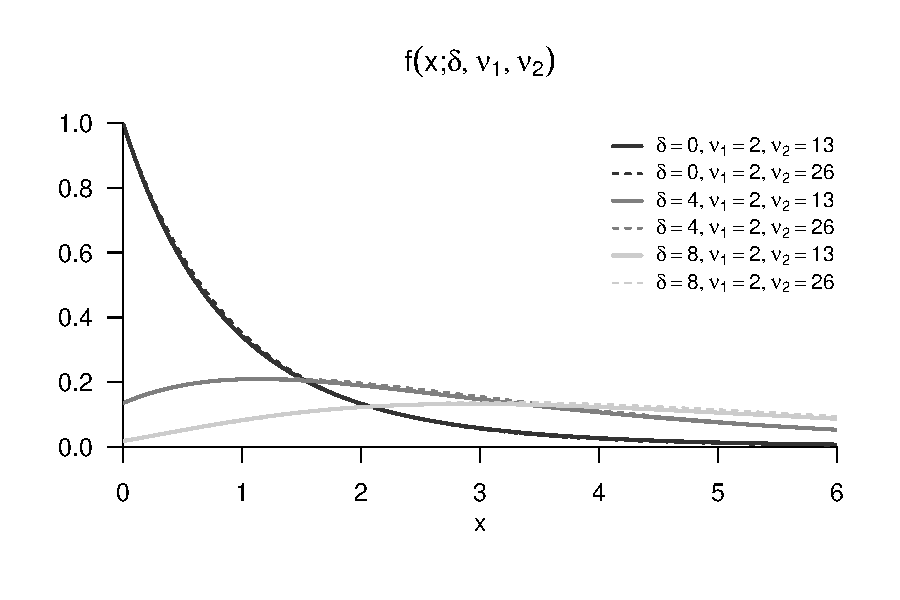
\includegraphics[width=0.8\linewidth]{8_Abbildungen/alm_8_f_nichtzentral_wdf} \end{center}
\end{frame}

\begin{frame}{F-Zufallsvariablen}
\protect\hypertarget{f-zufallsvariablen-5}{}
\small
\begin{theorem}[Nichtzentrale $F$-Transformation]
\justifying
\normalfont
$\zeta_1 \sim \chi^2(\delta,\nu_1)$ und $\zeta_2 \sim \chi^2(\nu_2)$ seien eine nichtzentrale $\chi^2$-
Zufallsvariable und eine  $\chi^2$-Zufallsvariable mit $\nu_1$ und $\nu_2$ Freiheitsgraden,
respektive und $\zeta_1$ und $\zeta_2$ seien unabhängig. Dann ist die Zufallsvariable
\begin{equation}
\xi := \frac{\zeta_1/\nu_1}{\zeta_2/\nu_2}
\end{equation}
eine nichtzentral $f$-verteilte Zufallsvariable mit Nichtzentralitätsparameter
$\delta$  und $\nu_1,\nu_2$ Freiheitsgraden, es gilt also $\xi \sim f(\delta, \nu_1,\nu_2)$.
\end{theorem}

\footnotesize

Bemerkungen

\begin{itemize}
\tightlist
\item
  Wir verzichten auf einen Beweis.
\end{itemize}
\end{frame}

\begin{frame}{}
\protect\hypertarget{section-10}{}
\vfill
\large
\setstretch{3}

F-Zufallsvariablen

\textbf{Likelihood-Quotienten-Statistiken}

Definition und Verteilung

Selbstkontrollfragen \vfill
\end{frame}

\begin{frame}{Likelihood-Quotienten-Statistiken}
\protect\hypertarget{likelihood-quotienten-statistiken}{}
\footnotesize
\begin{definition}[Likelihood-Quotienten-Statistik]
\justifying
Gegeben seien zwei parametrische statistische Modelle 
\begin{equation}
\mathcal{M}_0 := \left(\mathcal{Y},\mathcal{A}, \left\{\mathbb{P}^0_{\theta_0}|\theta_0 \in \Theta_0\right\}\right)
\mbox{ und }
\mathcal{M}_1 := \left(\mathcal{Y},\mathcal{A}, \left\{\mathbb{P}^1_{\theta_1}|\theta_1 \in \Theta_1\right\}\right)
\end{equation}
mit identischem Datenraum, identischer $\sigma$-Algebra und potentiell distinkten 
Wahrscheinlichkeitsmaßmengen und Parameterräumen. Sei weiterhin $\upsilon$ 
ein Zufallsvektor mit Datenraum $\mathcal{Y}$. Seien schließlich $L_0^\upsilon$ 
und $L_1^\upsilon$ die Likelihood-Funktionen von $\mathcal{M}_0$ und $\mathcal{M}_1$, 
respektive, wobei das Superskript $^\upsilon$ jeweils an die Datenabhängigkeit 
der Likelihood Funktion erinnern soll. Dann wird 
\begin{equation}
\Lambda := \frac{\max_{\theta_0 \in \Theta_0}L^\upsilon_0(\theta_0)}{\max_{\theta_1 \in \Theta_1}L^\upsilon_1(\theta_1)}, 
\end{equation}
\textit{Likelihood-Quotienten-Statistik} genannt.
\end{definition}
\end{frame}

\begin{frame}{Likelihood-Quotienten-Statistiken}
\protect\hypertarget{likelihood-quotienten-statistiken-1}{}
\footnotesize

Bemerkungen

\begin{itemize}
\item
  \justifying Eine Likelihood-Quotienten-Statistik setzt die
  Wahrscheinlichkeitsmassen/dichten eines beobachteten Datensatzes
  \(y \in \mathcal{Y}\) unter zwei statistischen Modellen \emph{nach
  Optimierung der jeweiligen Modellparameter} ins Verhältnis. Ein hoher
  Wert des Likelihood-Quotienten-Statistik entspricht einer höhereren
  Wahrscheinlichkeitsmasse/dichte des beobachteten Datensatzes
  \(y \in \mathcal{Y}\) unter \(\mathcal{M}_0\) als unter
  \(\mathcal{M}_1\) und vice versa.
\item
  \justifying  Die Wahrscheinlichkeitsdichten/massen beobachteter Daten
  nach Modellschätzung unter verschiedenen Modellen zu betrachten ist
  ein allgemeines Vorgehen zum Vergleich von Modellen. Letztlich erlaubt
  dieses Vorgehen, verschiedene wissenschaftliche Theorien über die
  Genese beobachtbarer Daten quantitativ zu vergleichen und die damit
  verbundene Unsicherheit zu quantifizieren.
\item
  \justifying  Modellvergleiche sind ein zentrales Thema in der
  Bayesianischen Inferenz die die Logik von
  Likelihood-Quotienten-Statistiken zum Beispiel unter den Begriffen der
  Bayes Factors oder der des Bayesian Information Criterions auf
  allgemeine probabilistische Modelle generalisiert. Allerdings sind,
  wie hier gesehen, Modellvergleiche auch im Rahmen der
  Frequentistischen Inferenz möglich und sinnvoll, Modellvergleiche sind
  also kein Alleinstellungsmerkmal der Bayesianischen gegenüber der
  Frequentistischen Inferenz.
\item
  Mit dem \emph{reduzierten Modell} und dem \emph{vollständigen Modell}
  betrachten wir im Folgenden zwei spezielle Formen von
  \(\mathcal{M}_0\) und \(\mathcal{M}_1\), respektive, im Kontext des
  ALMs.
\end{itemize}
\end{frame}

\begin{frame}{Likelihood-Quotienten-Statistiken}
\protect\hypertarget{likelihood-quotienten-statistiken-2}{}
\footnotesize
\begin{definition}[Vollständiges und reduziertes Modell]
Für $p > 1$ mit $p = p_0 + p_1$ seien
\begin{equation}
X := \begin{pmatrix} X_0 & X_1 \end{pmatrix}  \in \mathbb{R}^{n \times p}
\mbox{ mit }
X_0 \in \mathbb{R}^{n \times p_0}
\mbox{ und }
X_1 \in \mathbb{R}^{n \times p_1},
\end{equation}
sowie
\begin{equation}
\beta := \begin{pmatrix} \beta_0 \\ \beta_1 \end{pmatrix} \in \mathbb{R}^p
\mbox{ mit }
\beta_0 \in \mathbb{R}^{p_0}
\mbox{ und }
\beta_1 \in \mathbb{R}^{p_1}
\end{equation}
Partitionierungen einer $n \times p$ Designmatrix und eines $p$-dimensionalen
Betaparametervektors. Dann nennen wir
\begin{equation}
\upsilon = X\beta + \varepsilon \mbox{ mit } \varepsilon \sim N(0_n,\sigma^2I_n)
\end{equation}
das \textit{vollständige Modell} und
\begin{equation}
\upsilon = X_0\beta_0 + \varepsilon_0 \mbox{ mit } \varepsilon_0 \sim N(0_n,\sigma^2I_n)
\end{equation}
das \textit{reduzierte Modell} und sprechen von einer \textit{Partitionierung eines
(vollständigen) Modells}.
\end{definition}

Bemerkungen

\begin{itemize}
\tightlist
\item
  Man sagt auch, dass das reduzierte Modell im vollständigen Modell
  \textit{geschachtelt (nested)} ist.
\end{itemize}
\end{frame}

\begin{frame}{Likelihood-Quotienten-Statistiken}
\protect\hypertarget{likelihood-quotienten-statistiken-3}{}
\footnotesize
\begin{theorem}[Likelihood-Quotient von vollständigem und reduziertem Modell]
\justifying
\normalfont
Für $p = p_0 + p_1, p > 1$ sei eine Partitionierung eines vollständigen ALMs 
gegeben und es seien $\hat{\sigma}^2$ und $\hat{\sigma}^2_0$ die Maximum-Likelihood Schätzer
des Varianzparameters unter vollständigem und reduziertem Modell, respektive.
Weiterhin seien die zwei parametrischen statistischen Modelle $\mathcal{M}_0$ 
und $\mathcal{M}_1$ in der Definition der Likelihood-Quotienten-Statistik durch das 
reduzierte Modell und das vollständige Modell gegeben. 
Dann gilt
\begin{equation}
\Lambda = \left(\frac{\hat{\sigma}^2}{\hat{\sigma}_0^2}\right)^{\frac{n}{2}}
\end{equation}
\end{theorem}

Bemerkungen

\begin{itemize}
\tightlist
\item
  Informell gilt hier \begin{equation}
  \mathcal{M}_0 : \upsilon = X_0\beta_0 + \varepsilon_0 \mbox{ und } \mathcal{M}_1 : \upsilon = X\beta + \varepsilon
  \end{equation}
\end{itemize}
\end{frame}

\begin{frame}{Likelihood-Quotienten-Statistiken}
\protect\hypertarget{likelihood-quotienten-statistiken-4}{}
\footnotesize

\underline{Beweis}

Wir erinnern zunächst daran, dass die Maximum-Likelihood Schätzer des
Varianzparameters durch \begin{equation}
\hat{\sigma}^2 = \frac{1}{n}\left(\upsilon - X\hat{\beta}\right)^T\left(\upsilon - X\hat{\beta}\right)
\mbox{ und }
\hat{\sigma}^2_0 = \frac{1}{n}\left(\upsilon - X_0\hat{\beta}_0\right)^T\left(\upsilon - X_0\hat{\beta}_0\right)
\end{equation} respektive, gegeben sind, wobei \(\hat{\beta}\) und
\(\hat{\beta}_0\) die Maximum-Likelihood Schätzer der Betaparameter
unter vollständigem und reduziertem Modell, respektive, bezeichnen.
Weiterhin halten wir fest, dass für die Likelihood-Funktion des
vollständigem Modells an der Stelle der Maximum-Likelihood Schätzer
gilt, dass \begin{align}
\begin{split}
L^y_1(\hat{\beta}, \hat{\sigma}^2)
& = (2\pi)^{-\frac{n}{2}}(\hat{\sigma}^2)^{-\frac{n}{2}}\exp\left(-\frac{1}{2\hat{\sigma}^2}(y - X\hat{\beta})^T(y - X\hat{\beta})\right) \\
& = (2\pi)^{-\frac{n}{2}}(\hat{\sigma}^2)^{-\frac{n}{2}}\exp\left(-\frac{n}{2}\frac{(y - X\hat{\beta})^T(y - X\hat{\beta})}{(y - X\hat{\beta})^T(y - X\hat{\beta})}\right) \\
& = (2\pi)^{-\frac{n}{2}}(\hat{\sigma}^2)^{-\frac{n}{2}}e^{-\frac{n}{2}}
\end{split}
\end{align} und analog, dass für die Likelihood-Funktion des reduzierten
Modells an der Stelle der Maximum-Likelihood Schätzer gilt, dass
\begin{align}
\begin{split}
L^y_0(\hat{\beta}_0, \hat{\sigma}^2_0)
& = (2\pi)^{-\frac{n}{2}}(\hat{\sigma}^2_0)^{-\frac{n}{2}}e^{-\frac{n}{2}}
\end{split}
\end{align} Damit ergibt sich dann aber \begin{equation*}
\Lambda 
= \frac{\max_{\theta_0 \in \Theta_0}L^\upsilon_0(\theta_0)}{\max_{\theta_1 \in \Theta_1}L^\upsilon_1(\theta_1)} 
= \frac{L^\upsilon_0(\hat{\beta}_0, \hat{\sigma}_0^2)}{L^\upsilon_1(\hat{\beta}, \hat{\sigma}^2)}
= \frac{(2\pi)^{-\frac{n}{2}}(\hat{\sigma}^2_0)^{-\frac{n}{2}}e^{-\frac{n}{2}}}{(2\pi)^{-\frac{n}{2}}(\hat{\sigma}^2)^{-\frac{n}{2}}e^{-\frac{n}{2}}}
= \left(\frac{\hat{\sigma}^2_0}{\hat{\sigma}^2}\right)^{-\frac{n}{2}}
= \left(\frac{\hat{\sigma}^2}{\hat{\sigma}^2_0}\right)^{\frac{n}{2}}
\end{equation*}
\end{frame}

\begin{frame}{}
\protect\hypertarget{section-11}{}
\vfill
\large
\setstretch{3}

F-Zufallsvariablen

Likelihood-Quotienten

\textbf{Definition und Verteilung}

Selbstkontrollfragen \vfill
\end{frame}

\begin{frame}{Definition und Verteilung}
\protect\hypertarget{definition-und-verteilung}{}
\footnotesize
\begin{definition}[F-Statistik]
Für $X \in \mathbb{R}^{n \times p}, \beta \in \mathbb{R}^p$ und $\sigma^2 > 0$
sei ein ALM der Form
\begin{equation}
\upsilon = X\beta + \varepsilon \mbox{ mit } \varepsilon \sim N(0_n,\sigma^2I_n)
\end{equation}
mit der Partitionierung
\begin{equation}
X      = \begin{pmatrix} X_0     & X_1      \end{pmatrix},
X_0      \in \mathbb{R}^{n\times p_0},
X_1      \in \mathbb{R}^{n\times p_1},
\mbox{ und }
\beta := \begin{pmatrix} \beta_0 \\ \beta_1 \end{pmatrix},
\beta_0 \in \mathbb{R}^{p_0},
\beta_1 \in \mathbb{R}^{p_1},
\end{equation}
mit $p = p_0 + p_1$ gegeben. Weiterhin seien mit
\begin{equation}
\hat{\beta}_0 := (X_0^TX_0)^{-1} X_0^T\upsilon \mbox{ und } \hat{\beta} := (X^TX)^{-1}X^T\upsilon
\end{equation}
die Residuenvektoren
\begin{equation}
\hat{\varepsilon}_0 := \upsilon - X_0\hat{\beta}_0 \mbox{ und } \hat{\varepsilon} := \upsilon - X\hat{\beta}
\end{equation}
definiert. Dann ist die F-Statistik definiert als
\begin{equation}
F := \frac{(\hat{\varepsilon}_0^T\hat{\varepsilon}_0-\hat{\varepsilon}^T\hat{\varepsilon})/p_1}{\hat{\varepsilon}^T\hat{\varepsilon}/(n-p)}
\end{equation}
\end{definition}
\end{frame}

\begin{frame}{Definition und Verteilung}
\protect\hypertarget{definition-und-verteilung-1}{}
\footnotesize

Bemerkungen

\begin{itemize}
\tightlist
\item
  \justifying Der Zähler der F-Statistik \begin{equation}
  \frac{\hat{\varepsilon}_0^T\hat{\varepsilon}_0 - \hat{\varepsilon}^T\hat{\varepsilon}}{p_1}
  \end{equation} misst, inwieweit die \(p_1\) Regressoren in \(X_1\) die
  Residualquadratsumme reduzieren und zwar im Verhältnis zur Anzahl
  dieser Regressoren. Das heißt, dass bei gleicher Größe der
  Residualquadratsummenreduktion (und gleichem Nenner) ein größerer
  \(F\) Wert resultiert, wenn diese durch weniger zusätzliche
  Regressoren resultiert, also \(p_1\) klein ist (und vice versa). Im
  Sinne der Anzahl der Spalten von \(X\) und der entsprechenden
  Komponenten von \(\beta\) favorisiert die \(F\)-Statistik also weniger
  ``komplexe'' Modelle.
\item
  Für den Nenner der F-Statistik gilt \begin{equation}
  \frac{\hat{\varepsilon}^T\hat{\varepsilon}}{n-p} = \hat{\sigma}^2,
  \end{equation} wobei \(\hat{\sigma}^2\) hier der aufgrund des
  vollständigen Modells geschätzte Schätzer von \(\sigma^2\) ist. Werden
  die Daten tatsächlich unter dem reduzierten Modell generiert, so kann
  das vollständige Modell dies durch \(\hat{\beta}_1 \approx 0_{p_1}\)
  abbilden und erreicht eine ähnliche \(\sigma^2\) Schätzung wie das
  reduzierte Modell. Werden die Daten de-facto unter dem vollständigem
  Modell generiert, so ist
  \(\hat{\varepsilon}^T\hat{\varepsilon}/(n-p)\) ein besserer Schätzer
  von \(\sigma^2\) als
  \(\hat{\varepsilon}^T_0\hat{\varepsilon_0}/(n-p)\), da sich für diesen
  Datenvariabilität, die nicht durch die \(p_0\) Regressoren in \(X_0\)
  erklärt wird, in der Schätzung von \(\sigma^2\) widerspiegeln würde.
  Der Nenner der F-Statistik ist also in beiden Fällen der sinnvollere
  Schätzer von \(\sigma^2\).
\item
  Zusammengenommen misst die F-Statistik also die
  Residualquadratsummenreduktion durch die \(p_1\) Regressoren in
  \(X_1\) gegenüber den \(p_0\) Regressoren in \(X_0\) pro
  Datenvariabilitäts (\(\sigma^2\))- und Regressor (\(p_1\))-Einheit.
\end{itemize}
\end{frame}

\begin{frame}{Definition und Verteilung}
\protect\hypertarget{definition-und-verteilung-2}{}
\vspace{2mm}
\footnotesize
\begin{theorem}[F-Statistik und Likelihood-Quotienten-Statistik]
\justifying
\normalfont
Es sei die Partitionierung eines ALMs in ein vollständiges und ein reduziertes Modell
gegeben und $F$ und $\Lambda$ seien die entsprechenden F- und Likelihood-Quotienten-Statistiken. 
Dann gilt
\begin{equation}
F = \frac{n-p}{p_1}\left(\Lambda^{-\frac{2}{n}} -1 \right).
\end{equation}
\end{theorem}
\vspace{-2mm}

Bemerkungen

\begin{itemize}
\tightlist
\item
  Zwischen der F- und der Likelihood-Quotienten-Statistik besteht ein
  funktionaler reziproker Zusammenhang.
\item
  Für \(\Lambda = 1\) gilt \(F = 0\).
\item
  Wir visualisieren den funktionalen Zusammenhang für
  \(n = 12, p = 2, p_1 = 1\) untenstehend.
\end{itemize}

\vspace{-2mm}

\begin{center}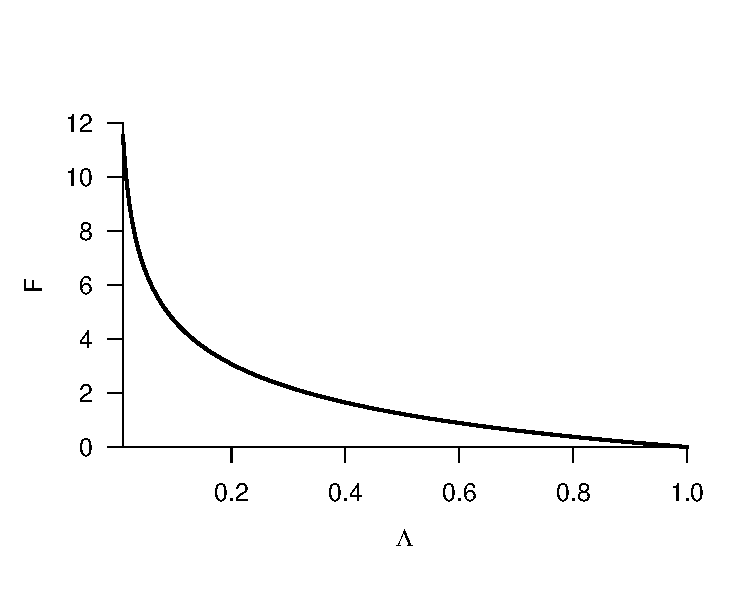
\includegraphics[width=0.5\linewidth]{8_Abbildungen/alm_8_F_Lambda} \end{center}
\end{frame}

\begin{frame}{Definition und Verteilung}
\protect\hypertarget{definition-und-verteilung-3}{}
\footnotesize

\underline{Beweis}

Wir erinnern zunächst daran, dass die Maximum-Likelihood Schätzer des
Varianzparameters durch \begin{equation}
\hat{\sigma}^2 = \frac{1}{n}\left(\upsilon - X\hat{\beta}\right)^T\left(\upsilon - X\hat{\beta}\right) = \frac{\hat{\varepsilon}^T\hat{\varepsilon}}{n}
\mbox{ und }
\hat{\sigma}^2_0 = \frac{1}{n}\left(\upsilon - X_0\hat{\beta}_0\right)^T\left(\upsilon - X_0\hat{\beta}_0\right) = \frac{\hat{\varepsilon}^T_0\hat{\varepsilon}_0}{n}
\end{equation} gegeben sind. Mit der Definition der F-Statistik und der
Form der Likelihood-Quotienten-Statistik für den Vergleich von
reduziertem und vollständigem Modell ergibt sich dann \begin{align}
\begin{split}
F 
& = \frac{(\hat{\varepsilon}_0^T\hat{\varepsilon}_0 - \hat{\varepsilon}^T\hat{\varepsilon})/p_1}{\hat{\varepsilon}^T\hat{\varepsilon}/(n-p)} \\
& = \frac{n(\hat{\sigma}^2_0 - \hat{\sigma}^2)/p_1}{n\hat{\sigma}^2/(n-p)} \\
& = \frac{n-p}{p_1} \frac{\hat{\sigma}^2_0 - \hat{\sigma}^2 }{\hat{\sigma}^2} \\
& = \frac{n-p}{p_1} \left(\frac{\hat{\sigma}^2_0}{\hat{\sigma}^2} - \frac{\hat{\sigma}^2}{\hat{\sigma}^2} \right)  \\
& = \frac{n-p}{p_1} \left(\Lambda^{-\frac{2}{n}} - 1\right)
\end{split}
\end{align}
\end{frame}

\begin{frame}[fragile]{Definition und Verteilung}
\protect\hypertarget{definition-und-verteilung-4}{}
\vspace{1mm}
\setstretch{.9}
\small

Beispiel (1) Einfache lineare Regression \footnotesize \begin{equation}
X = \begin{pmatrix} X_0 & X_1 \end{pmatrix}, X_0 := 1_{n}, X_1 := (x_1,...,x_n)^T,
\beta  := \begin{pmatrix} \beta_0 \\ \beta_1 \end{pmatrix},
\beta_0 = \mbox{Interzept,  }
\beta_1 = \mbox{Steigung }
\end{equation} \tiny

\begin{Shaded}
\begin{Highlighting}[]
\CommentTok{\# Modellformulierung}
\FunctionTok{library}\NormalTok{(MASS)                                             }\CommentTok{\# Multivariate Normalverteilung}
\NormalTok{nmod   }\OtherTok{=} \DecValTok{2}                                                \CommentTok{\# Anzahl Modelle}
\NormalTok{n      }\OtherTok{=} \DecValTok{10}                                               \CommentTok{\# Anzahl Datenpunkte}
\NormalTok{p      }\OtherTok{=} \DecValTok{2}                                                \CommentTok{\# Anzahl Betaparameter}
\NormalTok{p\_0    }\OtherTok{=} \DecValTok{1}                                                \CommentTok{\# Anzahl Betaparameter reduziertes Modell}
\NormalTok{p\_1    }\OtherTok{=} \DecValTok{1}                                                \CommentTok{\# Anzahl zusätzlicher Betaparameter vollständiges Modell}
\NormalTok{p      }\OtherTok{=}\NormalTok{ p\_0 }\SpecialCharTok{+}\NormalTok{ p\_1                                        }\CommentTok{\# Anzahl Betaparameter im vollständigem Modell}
\NormalTok{x      }\OtherTok{=} \DecValTok{1}\SpecialCharTok{:}\NormalTok{n                                              }\CommentTok{\# Prädiktorwerte}
\NormalTok{X      }\OtherTok{=} \FunctionTok{matrix}\NormalTok{(}\FunctionTok{c}\NormalTok{(}\FunctionTok{rep}\NormalTok{(}\DecValTok{1}\NormalTok{,n),x), }\AttributeTok{nrow =}\NormalTok{ n)                  }\CommentTok{\# Designmatrix des vollständigen Modells}
\NormalTok{X\_0    }\OtherTok{=}\NormalTok{ X[,}\DecValTok{1}\NormalTok{]                                            }\CommentTok{\# Designmatrix des reduzierten Modells}
\NormalTok{I\_n    }\OtherTok{=} \FunctionTok{diag}\NormalTok{(n)                                          }\CommentTok{\# n x n Einheitsmatrix}
\NormalTok{beta   }\OtherTok{=} \FunctionTok{matrix}\NormalTok{(}\FunctionTok{c}\NormalTok{(}\DecValTok{1}\NormalTok{,}\DecValTok{0}\NormalTok{,}\DecValTok{1}\NormalTok{,.}\DecValTok{5}\NormalTok{), }\AttributeTok{nrow =} \DecValTok{2}\NormalTok{)                    }\CommentTok{\# wahre , aber unbekannte , Betaparameter}
\NormalTok{nscn   }\OtherTok{=} \FunctionTok{ncol}\NormalTok{(beta)                                       }\CommentTok{\# Anzahl wahrer, aber unbekannter, Hypothesenszenarien}
\NormalTok{sigsqr }\OtherTok{=} \DecValTok{1}                                                \CommentTok{\# wahrer, aber unbekannter, Varianzparameter}

\CommentTok{\# Modellsimulation und Evaluierung}
\NormalTok{Eff    }\OtherTok{=} \FunctionTok{matrix}\NormalTok{(}\FunctionTok{rep}\NormalTok{(}\ConstantTok{NaN}\NormalTok{, nscn), }\AttributeTok{nrow =}\NormalTok{ nscn)              }\CommentTok{\# F{-}Statistiik Realisierungsarray}
\ControlFlowTok{for}\NormalTok{(s }\ControlFlowTok{in} \DecValTok{1}\SpecialCharTok{:}\NormalTok{nscn)\{                                         }\CommentTok{\# Szenarieniterationen}
\NormalTok{  y               }\OtherTok{=} \FunctionTok{mvrnorm}\NormalTok{(}\DecValTok{1}\NormalTok{, X }\SpecialCharTok{\%*\%}\NormalTok{beta[,s], sigsqr}\SpecialCharTok{*}\NormalTok{I\_n) }\CommentTok{\# Datenrealisierung}
\NormalTok{  beta\_hat\_0      }\OtherTok{=} \FunctionTok{solve}\NormalTok{(}\FunctionTok{t}\NormalTok{(X\_0)}\SpecialCharTok{\%*\%}\NormalTok{X\_0)}\SpecialCharTok{\%*\%}\FunctionTok{t}\NormalTok{(X\_0)}\SpecialCharTok{\%*\%}\NormalTok{y      }\CommentTok{\# Betaparameterschätzer reduziertes Modell}
\NormalTok{  beta\_hat        }\OtherTok{=} \FunctionTok{solve}\NormalTok{(}\FunctionTok{t}\NormalTok{(X)  }\SpecialCharTok{\%*\%}\NormalTok{X  )}\SpecialCharTok{\%*\%}\FunctionTok{t}\NormalTok{(X)  }\SpecialCharTok{\%*\%}\NormalTok{y      }\CommentTok{\# Betaparameterschätzer vollständiges Modell}
\NormalTok{  eps\_0\_hat       }\OtherTok{=}\NormalTok{ y}\SpecialCharTok{{-}}\NormalTok{X\_0}\SpecialCharTok{\%*\%}\NormalTok{beta\_hat\_0                    }\CommentTok{\# Residuenvektor reduziertes Modell}
\NormalTok{  eps\_hat         }\OtherTok{=}\NormalTok{ y}\SpecialCharTok{{-}}\NormalTok{X}\SpecialCharTok{\%*\%}\NormalTok{beta\_hat                        }\CommentTok{\# Residuenvektor vollständiges Modell}
\NormalTok{  eps\_0\_eps\_0\_hat }\OtherTok{=} \FunctionTok{t}\NormalTok{(eps\_0\_hat) }\SpecialCharTok{\%*\%}\NormalTok{ eps\_0\_hat            }\CommentTok{\# RQS reduziertes Modell}
\NormalTok{  eps\_eps\_hat     }\OtherTok{=} \FunctionTok{t}\NormalTok{(eps\_hat)   }\SpecialCharTok{\%*\%}\NormalTok{ eps\_hat              }\CommentTok{\# RQS vollständiges Modell}
\NormalTok{  Eff[s]          }\OtherTok{=}\NormalTok{ (((eps\_0\_eps\_0\_hat}\SpecialCharTok{{-}}\NormalTok{eps\_eps\_hat)}\SpecialCharTok{/}\NormalTok{p\_1)}\SpecialCharTok{/} \CommentTok{\# F{-}Statistik}
\NormalTok{                       (eps\_eps\_hat}\SpecialCharTok{/}\NormalTok{(n}\SpecialCharTok{{-}}\NormalTok{p)))\}}
\end{Highlighting}
\end{Shaded}

\begin{verbatim}
> F-Statistik für beta_1  = 0_{p_1}: 0.357 
> F-Statistik für beta_1 != 0_{p_1}: 18.8
\end{verbatim}
\end{frame}

\begin{frame}{Definition und Verteilung}
\protect\hypertarget{definition-und-verteilung-5}{}
\footnotesize
\begin{theorem}[F-Statistik]
\justifying
\normalfont
Für $X \in \mathbb{R}^{n \times p}, \beta \in \mathbb{R}^p$ und $\sigma^2 > 0$
sei ein ALM der Form
\begin{equation}
\upsilon = X\beta + \varepsilon \mbox{ mit } \varepsilon \sim N(0_n,\sigma^2I_n)
\end{equation}
mit der Partitionierung
\begin{equation}
X      = \begin{pmatrix} X_0     & X_1      \end{pmatrix},
X_0      \in \mathbb{R}^{n\times p_0},
X_1      \in \mathbb{R}^{n\times p_1},
\mbox{ und }
\beta := \begin{pmatrix} \beta_0 \\ \beta_1 \end{pmatrix},
\beta_0 \in \mathbb{R}^{p_0},
\beta_1 \in \mathbb{R}^{p_1},
\end{equation}
mit $p = p_0 + p_1$ gegeben. Schließlich sei
\begin{equation}
c := \begin{pmatrix} 0_{p_0} \\ 1_{p_1} \end{pmatrix} \in \mathbb{R}^p
\end{equation}
ein Vektor. Dann gilt
\begin{equation}
F \sim f(\delta, p_1, n-p) \mbox{ mit } \delta := \frac{c^T\beta \left(c^T(X^TX)^{-1}c\right)^{-1}c^T \beta}{\sigma^2}
\end{equation}
\end{theorem}

Bemerkungen

\begin{itemize}
\tightlist
\item
  Wir verzichten auf einen Beweis.
\item
  \(F\) ist eine Funktion der Parameterschätzer, \(\delta\) ist eine
  Funktion der wahren, aber unbekannten, Parameter.
\item
  Diese Verteilung von \(F\) kann zum Nullhypothesentesten und zur
  Powerfunktionsevaluation genutzt werden.
\end{itemize}
\end{frame}

\begin{frame}[fragile]{Definition und Verteilung}
\protect\hypertarget{definition-und-verteilung-6}{}
\vspace{2mm}
\setstretch{.9}
\small

Beispiel (1) Einfache lineare Regression \footnotesize \begin{equation}
X = \begin{pmatrix} X_0 & X_1 \end{pmatrix}, X_0 := 1_{n}, X_1 := (x_1,...,x_n)^T,
\beta  := \begin{pmatrix} \beta_0 \\ \beta_1 \end{pmatrix},
\beta_0 = \mbox{Interzept,  }
\beta_1 = \mbox{Steigung }
\end{equation} \tiny

\begin{Shaded}
\begin{Highlighting}[]
\CommentTok{\# Modellformulierung}
\FunctionTok{library}\NormalTok{(MASS)                                               }\CommentTok{\# Multivariate Normalverteilung}
\NormalTok{nmod   }\OtherTok{=} \DecValTok{2}                                                  \CommentTok{\# Anzahl Modelle}
\NormalTok{n      }\OtherTok{=} \DecValTok{10}                                                 \CommentTok{\# Anzahl Datenpunkte}
\NormalTok{p\_0    }\OtherTok{=} \DecValTok{1}                                                  \CommentTok{\# Anzahl Betaparameter im reduzierten Modell}
\NormalTok{p\_1    }\OtherTok{=} \DecValTok{1}                                                  \CommentTok{\# Anzahl additiver Betaparameter im vollständigen Modell}
\NormalTok{p      }\OtherTok{=}\NormalTok{ p\_0 }\SpecialCharTok{+}\NormalTok{ p\_1                                          }\CommentTok{\# Anzahl Betaparameter im vollständigem Modell}
\NormalTok{x      }\OtherTok{=} \DecValTok{1}\SpecialCharTok{:}\NormalTok{n                                                }\CommentTok{\# Prädiktorwerte}
\NormalTok{X      }\OtherTok{=} \FunctionTok{matrix}\NormalTok{(}\FunctionTok{c}\NormalTok{(}\FunctionTok{rep}\NormalTok{(}\DecValTok{1}\NormalTok{,n),x), }\AttributeTok{nrow =}\NormalTok{ n)                    }\CommentTok{\# Designmatrix des vollständigen Modells}
\NormalTok{X\_0    }\OtherTok{=}\NormalTok{ X[,}\DecValTok{1}\NormalTok{]                                              }\CommentTok{\# Designmatrix des reduzierten Modells}
\NormalTok{I\_n    }\OtherTok{=} \FunctionTok{diag}\NormalTok{(n)                                            }\CommentTok{\# n x n Einheitsmatrix}
\NormalTok{beta   }\OtherTok{=} \FunctionTok{matrix}\NormalTok{(}\FunctionTok{c}\NormalTok{(}\DecValTok{1}\NormalTok{,}\DecValTok{0}\NormalTok{,}\DecValTok{1}\NormalTok{,.}\DecValTok{5}\NormalTok{), }\AttributeTok{nrow =} \DecValTok{2}\NormalTok{)                      }\CommentTok{\# wahre , aber unbekannte , Betaparameter}
\NormalTok{nscn   }\OtherTok{=} \FunctionTok{ncol}\NormalTok{(beta)                                         }\CommentTok{\# Anzahl wahrer, aber unbekannter, Hypothesenszenarien}
\NormalTok{sigsqr }\OtherTok{=} \DecValTok{1}                                                  \CommentTok{\# wahrer, aber unbekannter, Varianzparameter}
\NormalTok{c      }\OtherTok{=} \FunctionTok{matrix}\NormalTok{((}\FunctionTok{c}\NormalTok{(}\DecValTok{0}\NormalTok{,}\DecValTok{1}\NormalTok{)), }\AttributeTok{nrow =} \DecValTok{2}\NormalTok{)                         }\CommentTok{\# Vektor  }

\CommentTok{\# Frequentistische Simulation}
\NormalTok{nsim   }\OtherTok{=} \FloatTok{1e4}                                                \CommentTok{\# Anzahl Realisierungen des n{-}dimensionalen ZVs}
\NormalTok{delta  }\OtherTok{=} \FunctionTok{rep}\NormalTok{(}\ConstantTok{NaN}\NormalTok{,nscn)                                      }\CommentTok{\# Nichtzentralitätsparameterarray}
\NormalTok{Eff    }\OtherTok{=} \FunctionTok{matrix}\NormalTok{(}\FunctionTok{rep}\NormalTok{(}\ConstantTok{NaN}\NormalTok{, nscn}\SpecialCharTok{*}\NormalTok{nsim), }\AttributeTok{nrow =}\NormalTok{ nscn)           }\CommentTok{\# F{-}Statistiik Realisierungsarray}
\ControlFlowTok{for}\NormalTok{(s }\ControlFlowTok{in} \DecValTok{1}\SpecialCharTok{:}\NormalTok{nscn)\{                                           }\CommentTok{\# Szenarieniterationen}
\NormalTok{  delta[s] }\OtherTok{=}\NormalTok{ (}\FunctionTok{t}\NormalTok{(}\FunctionTok{t}\NormalTok{(c)}\SpecialCharTok{\%*\%}\NormalTok{beta[,s])}\SpecialCharTok{\%*\%}                         \CommentTok{\# Nichtzentralitätsparameter}
              \FunctionTok{solve}\NormalTok{(}\FunctionTok{t}\NormalTok{(c)}\SpecialCharTok{\%*\%}\FunctionTok{solve}\NormalTok{(}\FunctionTok{t}\NormalTok{(X)}\SpecialCharTok{\%*\%}\NormalTok{X)}\SpecialCharTok{\%*\%}\NormalTok{c) }\SpecialCharTok{\%*\%}
\NormalTok{              (}\FunctionTok{t}\NormalTok{(c)}\SpecialCharTok{\%*\%}\NormalTok{beta[,s])}\SpecialCharTok{/}\NormalTok{sigsqr)}
  \ControlFlowTok{for}\NormalTok{(i }\ControlFlowTok{in} \DecValTok{1}\SpecialCharTok{:}\NormalTok{nsim)\{                                         }\CommentTok{\# Simulationsiterationen}
\NormalTok{    y               }\OtherTok{=} \FunctionTok{mvrnorm}\NormalTok{(}\DecValTok{1}\NormalTok{, X }\SpecialCharTok{\%*\%}\NormalTok{beta[,s], sigsqr}\SpecialCharTok{*}\NormalTok{I\_n) }\CommentTok{\# Datenrealisierung}
\NormalTok{    beta\_hat\_0      }\OtherTok{=} \FunctionTok{solve}\NormalTok{(}\FunctionTok{t}\NormalTok{(X\_0)}\SpecialCharTok{\%*\%}\NormalTok{X\_0)}\SpecialCharTok{\%*\%}\FunctionTok{t}\NormalTok{(X\_0)}\SpecialCharTok{\%*\%}\NormalTok{y      }\CommentTok{\# Betaparameterschätzer reduziertes Modell}
\NormalTok{    beta\_hat        }\OtherTok{=} \FunctionTok{solve}\NormalTok{(}\FunctionTok{t}\NormalTok{(X)  }\SpecialCharTok{\%*\%}\NormalTok{X  )}\SpecialCharTok{\%*\%}\FunctionTok{t}\NormalTok{(X)  }\SpecialCharTok{\%*\%}\NormalTok{y      }\CommentTok{\# Betaparameterschätzer vollständiges Modell}
\NormalTok{    eps\_0\_hat       }\OtherTok{=}\NormalTok{ y}\SpecialCharTok{{-}}\NormalTok{X\_0}\SpecialCharTok{\%*\%}\NormalTok{beta\_hat\_0                    }\CommentTok{\# Residuenvektor reduziertes Modell}
\NormalTok{    eps\_hat         }\OtherTok{=}\NormalTok{ y}\SpecialCharTok{{-}}\NormalTok{X}\SpecialCharTok{\%*\%}\NormalTok{beta\_hat                        }\CommentTok{\# Residuenvektor vollständiges Modell}
\NormalTok{    eps\_0\_eps\_0\_hat }\OtherTok{=} \FunctionTok{t}\NormalTok{(eps\_0\_hat) }\SpecialCharTok{\%*\%}\NormalTok{ eps\_0\_hat            }\CommentTok{\# RQS reduziertes Modell}
\NormalTok{    eps\_eps\_hat     }\OtherTok{=} \FunctionTok{t}\NormalTok{(eps\_hat)   }\SpecialCharTok{\%*\%}\NormalTok{ eps\_hat              }\CommentTok{\# RQS vollständiges Modell}
\NormalTok{    Eff[s,i]        }\OtherTok{=}\NormalTok{ (((eps\_0\_eps\_0\_hat}\SpecialCharTok{{-}}\NormalTok{eps\_eps\_hat)}\SpecialCharTok{/}\NormalTok{p\_1)}\SpecialCharTok{/} \CommentTok{\# F{-}Statistik}
\NormalTok{                         (eps\_eps\_hat}\SpecialCharTok{/}\NormalTok{(n}\SpecialCharTok{{-}}\NormalTok{p)))\}\}}
\end{Highlighting}
\end{Shaded}
\end{frame}

\begin{frame}{Definition und Verteilung}
\protect\hypertarget{definition-und-verteilung-7}{}
\vspace{1mm}

Beispiel (1) Einfache lineare Regression \vspace{2mm}

\vfill

\begin{center}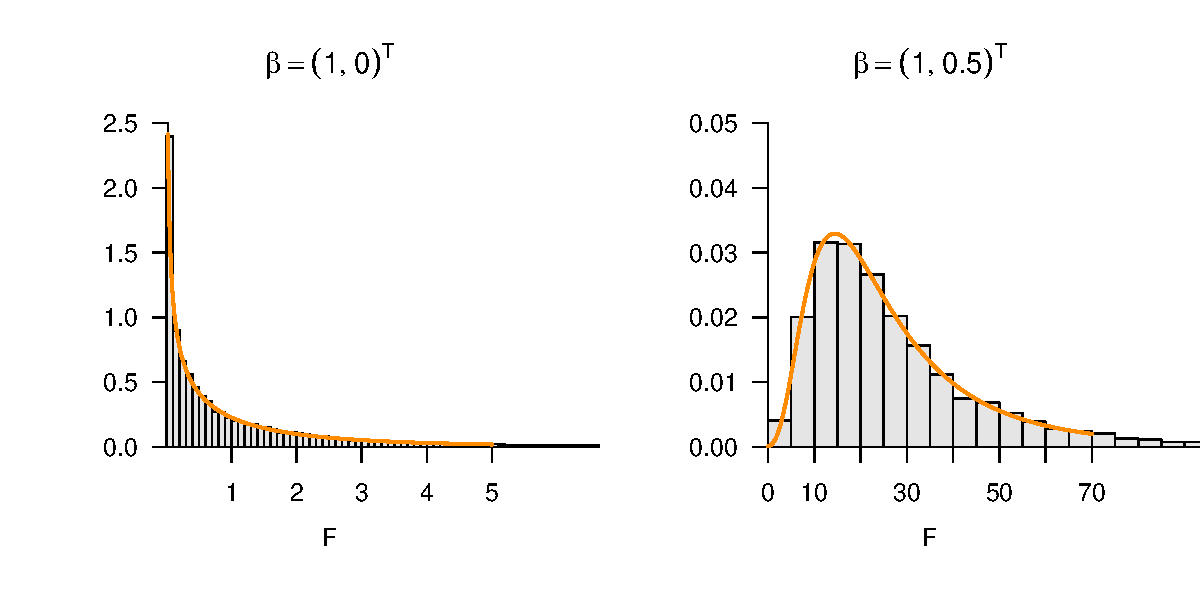
\includegraphics[width=1\linewidth]{8_Abbildungen/alm_8_F_Statistik} \end{center}
\vfill
\end{frame}

\begin{frame}{Definition und Verteilung}
\protect\hypertarget{definition-und-verteilung-8}{}
\small

Ausblick

\begin{itemize}
\item
  \justifying Die Theorie von T- und F-Statistiken wird unter dem
  Begriff der \emph{Allgemeinen Linearen Hypothese} verallgemeinert und
  integriert. Dabei betrachtet allgemeine lineare Funktionen der
  Betaparameter der Form \(C^T\beta\), wobei
  \(C \in \mathbb{R}^{p \times k}\) eine beliebige Matrix ist als
  Grundlage von Hypothesen. Zum Beispiel ergibt sich für
  \(C \in \mathbb{R}^{p \times 1}\) die hier und in Einheit (7)
  T-Statistiken betrachten Kontrastgewichtsvektoren. Im Kontext der
  \emph{Allgemeinen Linearen Hypothese} kann man weiterhin zeigen, dass
  \(F = T^2\), dass also auch das Quadrat einer T-Statistik
  \(f\)-verteilt ist und T-Statistiken damit (nur) spezielle
  F-Statistiken sind. \vspace{2mm}
\item
  \justifying Dennoch wird in der Anwendung sehr stark zwischen T- und
  F-Statistiken unterschieden und es ist sinnvoll, sich der
  unterschiedlichen Anwendungsfälle von T- und F-Statistiken bewusst zu
  sein. Gute Einführungen in die Theorie der Allgemeinen Linearen
  Hypothese bieten z.B. Searle (1971), Kapitel 3, Rencher and Schaalje
  (2008), Kapitel 8 oder Christensen (2011), Kapitel 3.
\end{itemize}
\end{frame}

\begin{frame}{}
\protect\hypertarget{section-12}{}
\vfill
\large
\setstretch{3}

F-Zufallsvariablen

Likelihood-Quotienten-Statistiken

Definition und Verteilung

\textbf{Selbstkontrollfragen} \vfill
\end{frame}

\begin{frame}{Selbstkontrollfragen}
\protect\hypertarget{selbstkontrollfragen}{}
\footnotesize
\setstretch{2.5}

\begin{enumerate}
\tightlist
\item
  Skizzieren Sie die \(f\)-Verteilung für \(\nu_1 = 2, \nu_2 = 13\) und
  \(\nu_1 = 4, \nu_2 = 13\).
\item
  Geben Sie die Definition der Likelihood-Quotienten-Statistik wieder.
\item
  Erläutern Sie die Definition der Likelihood-Quotienten-Statistik.
\item
  Geben Sie die Definition eines vollständigem und eines reduziertem
  ALMs wieder.
\item
  Geben Sie das Theorem zum Likelihood-Quotienten von vollständigem und
  reduzierten ALM wieder.
\item
  Definieren Sie die F-Statistik.
\item
  Erläutern Sie den Zähler der F-Statistik.
\item
  Erläutern Sie den Nenner der F-Statistik.
\item
  Erläutern Sie die F-Statistik.
\item
  Geben Sie das Theorem zum Zusammenhang von F-Statistik und
  Likelihood-Quotienten-Statistik wieder.
\end{enumerate}
\end{frame}

\begin{frame}{Referenzen}
\protect\hypertarget{referenzen}{}
\footnotesize

\hypertarget{refs}{}
\begin{CSLReferences}{1}{0}
\leavevmode\vadjust pre{\hypertarget{ref-christensen_2011}{}}%
Christensen, Ronald. 2011. \emph{Plane {Answers} to {Complex
Questions}}. Springer {Texts} in {Statistics}. {New York, NY}: {Springer
New York}. \url{https://doi.org/10.1007/978-1-4419-9816-3}.

\leavevmode\vadjust pre{\hypertarget{ref-rencher_2008}{}}%
Rencher, Alvin C., and G. Bruce Schaalje. 2008. \emph{Linear Models in
Statistics}. 2nd ed. {Hoboken, N.J}: {Wiley-Interscience}.

\leavevmode\vadjust pre{\hypertarget{ref-searle_1971}{}}%
Searle, S. R. 1971. \emph{Linear Models}. A {Wiley} Publication in
Mathematical Statistics. {New York}: {Wiley}.

\end{CSLReferences}
\end{frame}

\end{document}
